\documentclass[12pt,a4paper]{article}

\usepackage{polyglossia}
\usepackage{microtype}
\usepackage[margin=1in]{geometry}
\usepackage{graphicx}
\usepackage{multirow}
\usepackage{pbox}
\usepackage{graphicx}

\setdefaultlanguage{ukrainian}
\setotherlanguage{english}
\setmainfont[Ligatures=TeX]{Liberation Serif}
\setsansfont{Liberation Sans}
\setmonofont{Liberation Mono}

\begin{document}
\begin{titlepage}
  {\centering
	\Large НАЦІОНАЛЬНИЙ ТЕХНІЧНИЙ УНІВЕРСИТЕТ УКРАЇНИ\par
	\large «Київський політехнічний інститут імені Ігоря Сікорського»\par
	\vspace{1cm}
	Кафедра програмного забезпечення комп'ютерних систем\par
	\vspace{1cm}
	\normalsize Лабораторна робота \textnumero2\par
	із дисципліни «Операційні системи»\par
	\vspace{2cm}
	на тему: \textbf{ДОСЛІДЖЕННЯ РЕЖИМІВ РОБОТИ ОБЧИСЛЮВАЛЬНОЇ
	СИСТЕМИ ТА ОБРОБКИ ПЕРЕРИВАНЬ В ОС WINDOWS
	ЗА ДОПОМОГОЮ ОСНАСТКИ PERFORMANCE MONITOR}}
	\vspace{1cm}
	\begin{flushright}
	  Виконав:

		студент 2 курсу ФПМ групи КП-52

		\textit{Комар Григорій Миколайович}

		\vspace{1cm}

		Прийняла:

		\textit{к.т.н., ст. викл. Рибачок Наталія Антонівна}

		\textit{“28” листопада 2016р.}

		\vspace{1cm}
		\begin{tabular}{|l|l|}
		  \hline
			&Бали\\ \hline
			Якість виконання&\\ \hline
			Відповіді на питанняя&\\ \hline
			Оформлення звіту&\\ \hline
			Термін здачі&\\ \hline
			\multicolumn{1}{|r|}{Сумарний бал}&\\ \hline
		\end{tabular}
	\end{flushright}
	\vfill
	\centering КИЇВ — 2016
\end{titlepage}
\addtocounter{page}{1}

\textbf{Варіант завдання — взаємодія з графічним редактором.}

\begin{table}
  \begin{tabular}{|c|c|c|}
    \hline
    \multirow{2}{*}{Лічильник} & \multicolumn{2}{c|}{Середнє значення лічильника}\\ \cline{2-3}
    & відсутність взаємодії, \% & \pbox{4cm}{\centering взаємодія з обраним процесом,\%} \\ \hline
    Processor:\% Processor Time & 0.13  & 13.075 \\ \hline
    Processor: \% Idle Time & 99.97 & 86.925 \\ \hline
    Processor: \%Privileged Time & 0.091 & 1.86 \\ \hline
    Processor: \%User Time & 0.039 & 11.215 \\ \hline
    Process{\textbackslash}Idle: \%Privileged Time & 199.74 & 173.849 \\ \hline
    Process{\textbackslash}Idle:\% User Time & 0 & 0 \\ \hline
    Processor: Interrupts /sec & 154.538 & 281.192 \\ \hline
    Processor: \%Interrupt Time & 0.039 & 0.128 \\ \hline
    System: System Calls/sec & 1026.370 & 467 825.822 \\ \hline
    System: Exceptions/ Sec & 0.05 & 0.073 \\ \hline
  \end{tabular}
  \caption{Середнє значення лічильників}
\end{table}
\begin{table}
  \begin{tabular}{|c|c|c|c|}
    \hline
    \multirow{2}{*}{Лічильник} & \multicolumn{2}{c|}{Максимальне значення лічильника} & \multirow{2}{*}{\pbox{2.8cm}{\centering Тривалість перевищення, с}}\\ \cline{2-3}
    & \pbox{3cm}{\centering відсутність взаємодії, \%} & \pbox{3.5cm}{\centering взаємодія з обраним процесом, \%} & \\ \hline
    Processor:\% Processor Time & 0.938 & 24.844 & c \\ \hline
    Processor: Interrupts /sec & 272.05 & 324.104 & \\ \hline
    Processor: \%Interrupt Time & 0.156 & 0.313 & c \\ \hline
  \end{tabular}
  \caption{Максимальне значення лічильників}
\end{table}
Отже, при відсутності взаємодії з компьютером процессор майже весь час знаходиться в режимі простою, а час проведений в режимі користувача менший за час в режимі ядра. При взаємодії з графічним редактором зростає час проведений як в режимі ядра, так і в режимі користувача, однак час проведений в режимі користувача збільшився в 14 разів сильніше, ніж час проведений у режимі ядра. Взаємодія з графічним редактором відбувається переважно в режимі користувача. Кількість системних викликів за секунду значно зроса при взаємодії з графічним редактором. Отже, робота з графічним редактором вимагає від процесора великого об'єму обчислень які проводяться над оброблюваними графічними данними. Приріст часу в режимі ядра викликаний потребою в завантаженні файлу і обробці дій користувача з графічним інтерфейсом. Показники \textit{\%Processor Time, \%Interrupt Time, Interrupts/sec} не перевищували рекомендованого значаення.
\section*{Висновки}
Монітор продуктивності дозволяє аналізувати роботу ОС і запущених в ній процесів. В залежності від процесів, ОС може більшу частину часу знаходитись в режимі ядра або в режимі користувача. Процес Idle завжди виконується в режимі ядра. Взаємодія з апаратним забезпеченням, дії з графічним інтерфейсом і робота з файлами й системою вводу-виводу переводить виконання в режим ядра, тоді як безпосередньо обробка данним виконується в режимі користувача. Обробка вводу-виводу й дій користувача відбувається за допомогою переривань, і при інтенсивній роботі їх кількість зростає. Запущені процеси можуть взаємодіяти з ОС за допомогою системних викликів.

\begin{figure}[b] \centering
    \includegraphics[width=0.8485\textwidth]{"processor/1.png"}
  \caption{Робота процесору у режимах ядра та користувача під час простою}
\end{figure}
\begin{figure} \centering
    \includegraphics[width=0.8485\textwidth]{"processor/2.png"}
  \caption{Робота процесору у режимах ядра та користувача під час взаємодії з обраним процесом}
\end{figure}
\begin{figure} \centering
    \includegraphics[width=0.8485\textwidth]{"interrupts/1.png"}
  \caption{Робота операційної системи по обробці переривань під час простою}
\end{figure}
\begin{figure} \centering
    \includegraphics[width=0.8485\textwidth]{"interrupts/2.png"}
  \caption{Робота операційної системи по обробці переривань під час взаємодії з обраним процесом}
\end{figure}
\end{document}
